\chapter{WAF-A-MoLE++}
\label{chp:capitulo4}

Tendo em consideração o embasamento teórico estabelecido e o 
\section{Estruturação do Projeto}

\section{WAFs avaliados}

\subsection{WAF-Brain}

\textbf{Autores}: Sergio D Fdez, cr0hn, Enrique Garcia. Disponível no Github \href{https://github.com/BBVA}{BBVA}

O WAF-Brain foi um dos primeiros firewalls a serem testados pela equipe do WAF-A-MoLE, e subsequentemente é o primeiro modelo de exemplo disponibilizado para testes na documentação do mesmo. Dessa maneira, foi extensivamente testado com os novos operadores de mutação, sendo de grande ajuda para diagnosticar os incluídos no WAF-A-MoLE++.

\begin{figure}[ht]
    \centering
    \caption{Dependências e logomarca do WAF-Brain}
    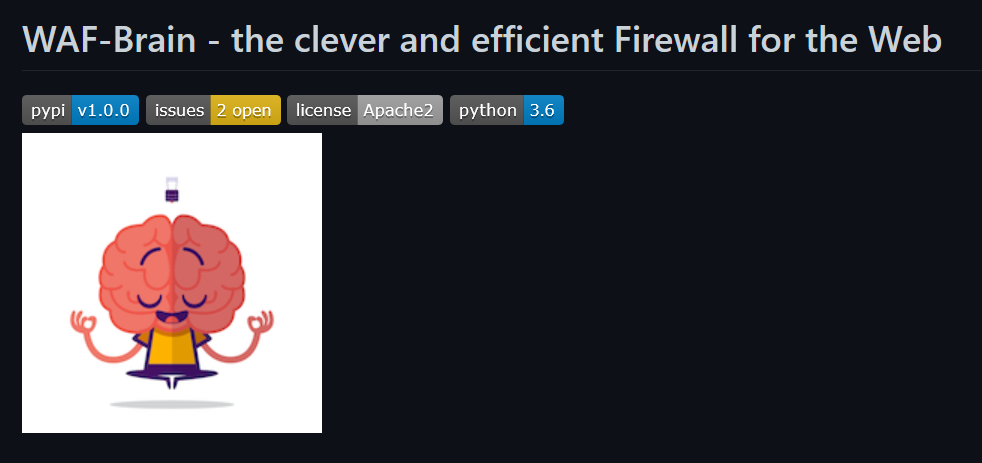
\includegraphics[width=12.5cm]{figuras/WAFBrain.png} 
    \legend{Fonte: \href{https://github.com/BBVA}{Github} (2019, p. TO-DO)}
    \label{fig:internet} 
\end{figure}

Seu funcionamento se dá, como anteriormente mencionado, através da estratégia de Deep Learning com Redes Neurais, pela qual são analisados cada campo de um determinado pedido HTTP sob a ótica de um classificador treinado desta maneira, determinando se esse campo é malicioso ou não.

Na adaptação WAF-A-MoLE, esse poder de predição é aproveitado exclusivamente na forma de probabilidade - tendo a probabilidade de ser uma SQL-Injection acima de um determinado limite, temos um caso malicioso. Isso requer que o classificador treinado no modelo não apenas mostre a previsão, mas também a precisa probabilidade com a qual chegou à mesma.

Por mais que se trate de um algoritmo sofisticado por natureza, surpreendentemente o WAF-Brain fora implementado pelos seus autores originais de uma maneira simplória o suficiente para ser um dos WAFs mais vulneráveis às estratégias de fuzzing do WAF-A-MoLE. Vários operadores de mutação isolados conseguem resultados frutíferos em pouco tempo, como será visto na seção de testes adiante.

\section{Operadores de Mutação}

\section{Modelos}
Todos os modelos implementados tiveram como base o firewall ML-Based-WAF, disponível por vladan-stojnic no \href{https://github.com/vladan-stojnic/ML-based-WAF}{Github} que fora o WAF open source mais promissor e mais plausível de adaptar. Sua performance também era factível no contexto de recursos disponíveis para a conclusão deste projeto final.

\begin{figure}[ht]
    \centering
    \caption{Repositório ML-Based-WAF}
    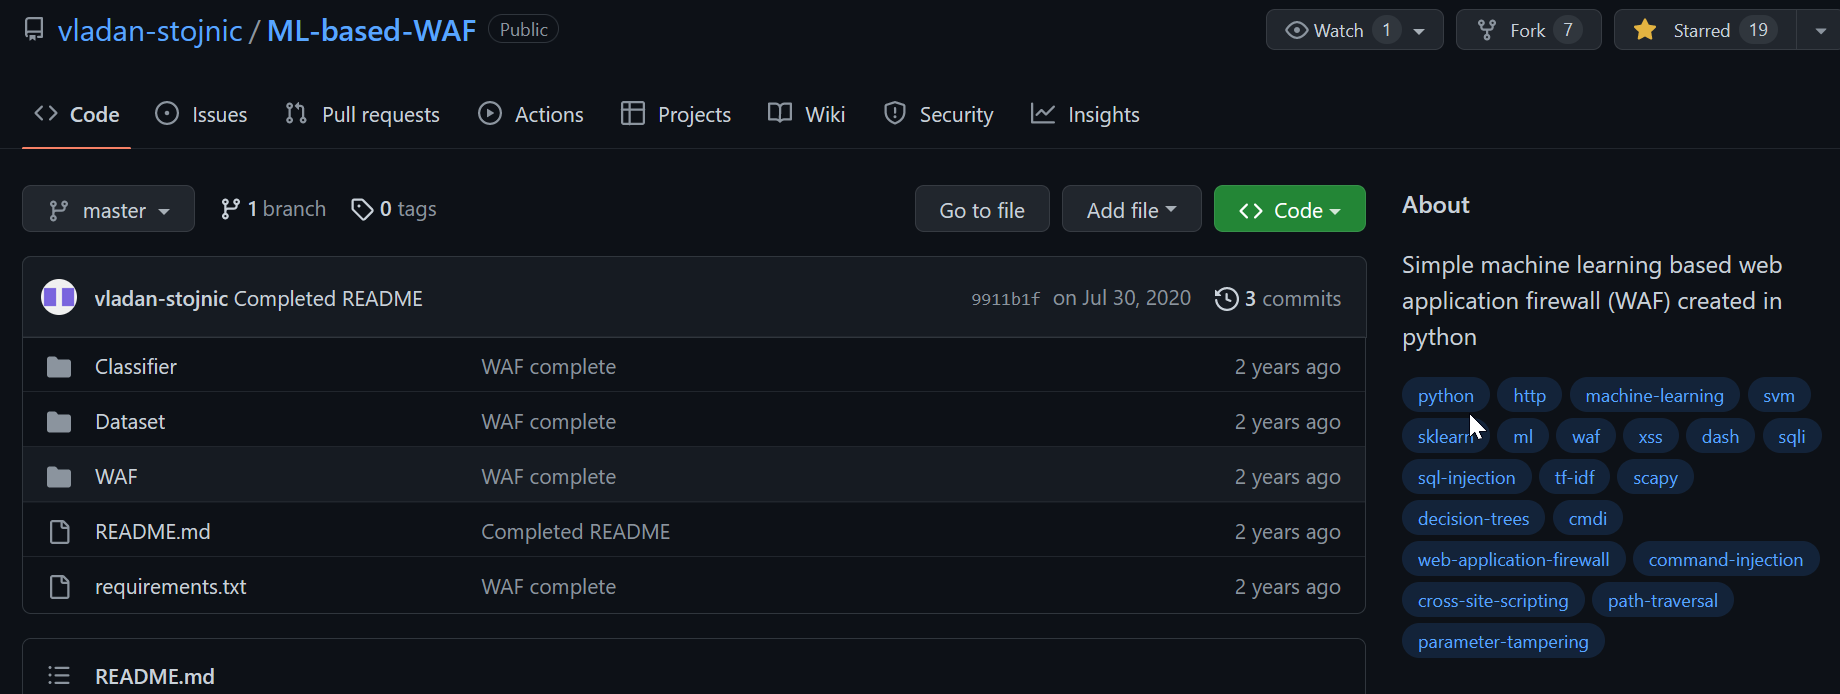
\includegraphics[width=16cm]{figuras/MLBasedWAF.png} 
    \legend{Fonte: \href{https://github.com/vladan-stojnic/ML-based-WAF}{Github} (2020, p. TO-DO)}
    \label{fig:internet} 
\end{figure}

Embora seja um WAF orientado ao tráfego real ou simulado de uma rede de fato, avaliando parâmetros HTTP em tempo real no seu componente sniffer.py tanto por SQL-Injections como por outras formas de ataque (XSS, cmdi e outras), ainda foi possível restringir seu funcionamento para adaptá-lo ao WAF-A-MoLE++. 

Para tal, foi necessário prever uma estratégia própria de treinamento para o classificador, além de um conjunto de dados especial para o mesmo. É cabível mencionar, no entanto, que isso introduziu uma série de dificuldades uma vez que sua documentação era consideravelmente modesta, e o banco novo a ser usado deveria seguir o padrão de formatação seguido pelo WAF.

Dentre as opções de datasets disponíveis com SQL Injections, foi escolhido inicialmente a versão SQLiV3.json da coleção do Kaggle que será amostrada a seguir.
Além disso, para corrigir uma variedade de erros de formatação, polir algumas queries incorretas (e de difícil proveito), e finalmente adaptar para o padrão .json utilizado pelo WAF, a seguinte função auxiliar foi codificada:

\begin{figure}[ht]
    \centering
    \caption{Detalhes Dataset SQL Injection Kaggle.}
    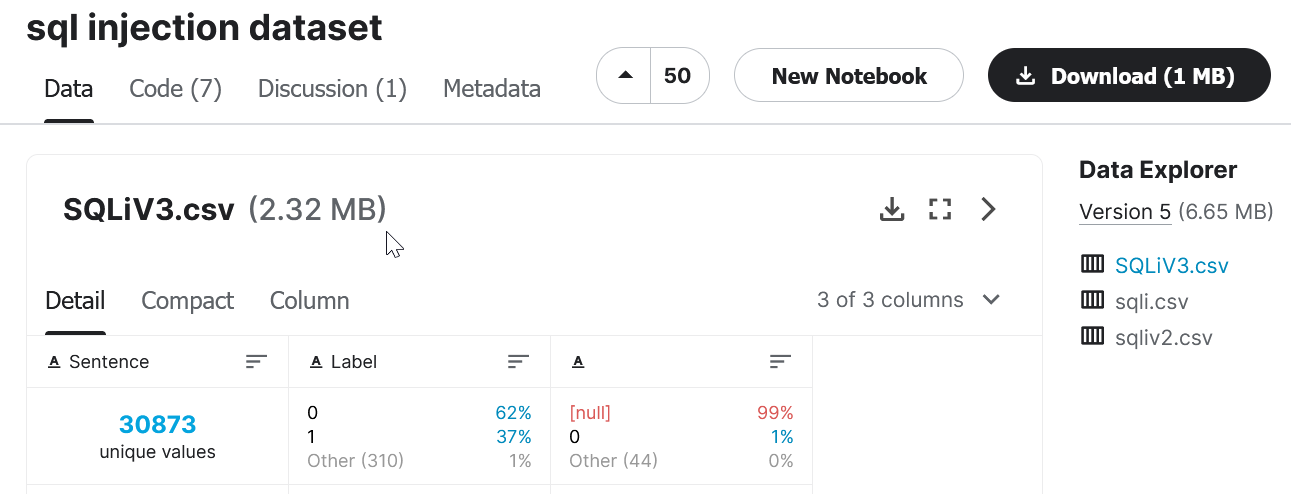
\includegraphics[width=16cm]{figuras/sqlInjectionDataset.png} 
    \legend{Fonte: \href{https://www.kaggle.com/datasets/syedsaqlainhussain/sql-injection-dataset}{Kaggle} (2021, p. TO-DO)}
    \label{fig:internet} 
\end{figure}

\label{sec:codigos}
\includecode[C]{Para tratamento de dados brutos} {alg:codigo3}{codigos/sqli_cleaner.py}

\subsection{Support Vector Machine}
Este foi o primeiro modelo implementado no WAF-A-MoLE++, antes do recebimento do dataset original da equipe original. 





